% Architecture diagram for the README.
% Build (macOS, uses the system Helvetica Neue):
%   tectonic docs/architecture.tex && pdftocairo -svg docs/architecture.pdf docs/architecture.svg
\documentclass[tikz,border=0pt]{standalone}
\usepackage{fontspec}
\setmainfont{Helvetica Neue}[BoldFont={Helvetica Neue Bold}, ItalicFont={Helvetica Neue Italic}]
\usetikzlibrary{positioning,fit,shapes.geometric,arrows.meta,backgrounds,calc}

\definecolor{ink}{HTML}{2F3437}
\definecolor{muted}{HTML}{787774}
\definecolor{line}{HTML}{CFCFCD}
\definecolor{canvas}{HTML}{FBFBFA}
\definecolor{blue}{HTML}{1F6C9F}
\definecolor{bluebg}{HTML}{E1F3FE}
\definecolor{green}{HTML}{346538}
\definecolor{greenbg}{HTML}{EDF3EC}
\definecolor{yellow}{HTML}{956400}
\definecolor{yellowbg}{HTML}{FBF3DB}

\tikzset{
  every node/.style={text=ink, font=\small},
  actor/.style={draw=yellow, fill=yellowbg, rounded corners=9pt, line width=0.8pt,
    minimum width=3.0cm, minimum height=1.1cm, align=center},
  svc/.style={draw=blue, fill=bluebg, rounded corners=3pt, line width=0.8pt,
    minimum width=4.0cm, minimum height=1.3cm, align=center},
  store/.style={cylinder, shape border rotate=90, aspect=0.22, draw=green, fill=greenbg,
    line width=0.8pt, minimum width=3.9cm, minimum height=1.7cm, align=center},
  box/.style={draw=line, fill=white, rounded corners=6pt, line width=0.8pt, inner sep=14pt},
  boxlabel/.style={anchor=south west, font=\footnotesize\bfseries, text=muted},
  flow/.style={-{Stealth[length=7pt]}, line width=0.9pt, draw=ink},
  lbl/.style={font=\footnotesize, text=muted, fill=canvas, inner sep=2pt},
  title/.style={font=\bfseries\small},
}

\pgfdeclarelayer{canvas}
\pgfsetlayers{canvas,background,main}

\begin{document}
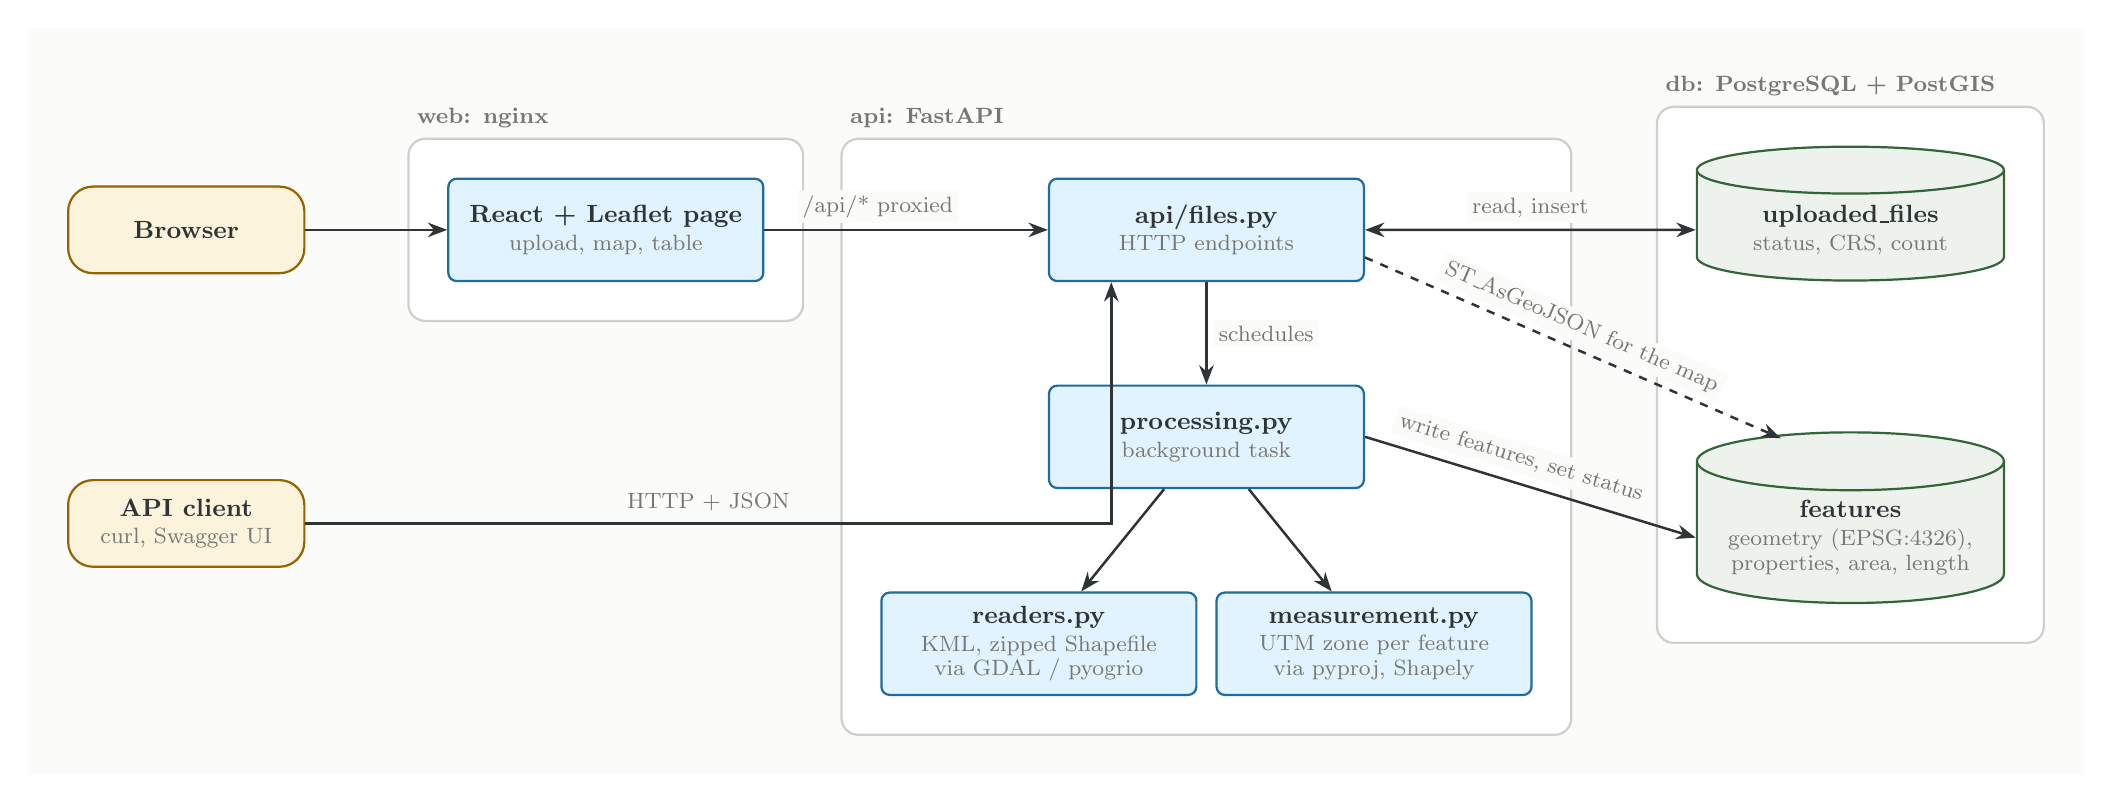
\begin{tikzpicture}[node distance=1.0cm and 1.6cm]

  % Clients
  \node[actor] (browser) {\textbf{Browser}};
  \node[actor, below=2.6cm of browser] (client) {\textbf{API client}\\[-1pt]{\footnotesize\color{muted}curl, Swagger UI}};

  % web container
  \node[svc, right=1.8cm of browser] (spa)
    {\textbf{React + Leaflet page}\\[-1pt]{\footnotesize\color{muted}upload, map, table}};

  % api container
  \node[svc, right=3.6cm of spa] (routes)
    {\textbf{api/files.py}\\[-1pt]{\footnotesize\color{muted}HTTP endpoints}};
  \node[svc, below=1.3cm of routes] (processing)
    {\textbf{processing.py}\\[-1pt]{\footnotesize\color{muted}background task}};
  \node[svc, below left=1.3cm and -1.9cm of processing] (readers)
    {\textbf{readers.py}\\[-1pt]{\footnotesize\color{muted}KML, zipped Shapefile}\\[-2pt]{\footnotesize\color{muted}via GDAL / pyogrio}};
  \node[svc, below right=1.3cm and -1.9cm of processing] (measurement)
    {\textbf{measurement.py}\\[-1pt]{\footnotesize\color{muted}UTM zone per feature}\\[-2pt]{\footnotesize\color{muted}via pyproj, Shapely}};

  % db container
  \node[store, right=4.2cm of routes] (files)
    {\textbf{uploaded\_files}\\[-1pt]{\footnotesize\color{muted}status, CRS, count}};
  \node[store, below=1.9cm of files] (features)
    {\textbf{features}\\[-1pt]{\footnotesize\color{muted}geometry (EPSG:4326),}\\[-2pt]{\footnotesize\color{muted}properties, area, length}};

  % Containers, drawn behind the nodes
  \begin{scope}[on background layer]
    \node[box, fit=(spa)] (webbox) {};
    \node[box, fit=(routes)(processing)(readers)(measurement)] (apibox) {};
    \node[box, fit=(files)(features)] (dbbox) {};
  \end{scope}
  \node[boxlabel] at (webbox.north west) {web: nginx};
  \node[boxlabel] at (apibox.north west) {api: FastAPI};
  \node[boxlabel] at (dbbox.north west) {db: PostgreSQL + PostGIS};

  % Flows
  \draw[flow] (browser) -- (spa);
  \draw[flow] (spa) -- node[lbl, above=2pt, pos=0.4] {/api/* proxied} (routes);
  \draw[flow] (client.east) -| ($(routes.south west)!0.2!(routes.south east)$)
    node[lbl, pos=0.25, above=2pt] {HTTP + JSON};
  \draw[flow] (routes) -- node[lbl, right=2pt] {schedules} (processing);
  \draw[flow] (processing) -- (readers);
  \draw[flow] (processing) -- (measurement);
  \draw[flow, {Stealth[length=7pt]}-{Stealth[length=7pt]}] (routes) -- node[lbl, above=2pt] {read, insert} (files);
  \draw[flow] (processing.east) -- node[lbl, above=3pt, sloped, pos=0.45] {write features, set status} (features.west);
  \draw[flow, dashed] (routes.east) ++(0,-0.35) -- node[lbl, above=2pt, sloped, pos=0.5] {ST\_AsGeoJSON for the map} ($(features.north west)!0.15!(features.north east)$);

  % Canvas, below the container boxes
  \begin{pgfonlayer}{canvas}
    \fill[canvas] ($(current bounding box.south west)+(-0.5,-0.5)$) rectangle ($(current bounding box.north east)+(0.5,0.5)$);
  \end{pgfonlayer}
\end{tikzpicture}
\end{document}
